%\documentclass[portrait,final,a0paper]{baposter}
\documentclass[a0paper,portrait,final]{baposter}
% Usa a4shrink for an a4 sized paper.

\tracingstats=2

\usepackage{calc}
\usepackage{graphicx}
\usepackage{amsmath}
\usepackage{amssymb}
\usepackage{relsize}
\usepackage{multirow}
\usepackage{bm}

\usepackage{graphicx}
\usepackage{multicol}

\usepackage{pgfbaselayers}
\pgfdeclarelayer{background}
\pgfdeclarelayer{foreground}
\pgfsetlayers{background,main,foreground}

\usepackage{times}
\usepackage{helvet}
%\usepackage{bookman}
\usepackage{palatino}

\newcommand{\captionfont}{\footnotesize}

\selectcolormodel{cmyk}

\graphicspath{{images/}}


%%%%%%%%%%%%%%%%%%%%%%%%%%%%%%%%%%%%%%%%%%%%%%%%%%%%%%%%%%%%%%%%%%%%%%%%%%%%%%%%
%%%% Some math symbols used in the text
%%%%%%%%%%%%%%%%%%%%%%%%%%%%%%%%%%%%%%%%%%%%%%%%%%%%%%%%%%%%%%%%%%%%%%%%%%%%%%%%
% Format 
\newcommand{\Matrix}[1]{\begin{bmatrix} #1 \end{bmatrix}}
\newcommand{\Vector}[1]{\Matrix{#1}}
\newcommand*{\SET}[1]  {\ensuremath{\mathcal{#1}}}
\newcommand*{\MAT}[1]  {\ensuremath{\mathbf{#1}}}
\newcommand*{\VEC}[1]  {\ensuremath{\bm{#1}}}
\newcommand*{\CONST}[1]{\ensuremath{\mathit{#1}}}
\newcommand*{\norm}[1]{\mathopen\| #1 \mathclose\|}% use instead of $\|x\|$
\newcommand*{\abs}[1]{\mathopen| #1 \mathclose|}% use instead of $\|x\|$
\newcommand*{\absLR}[1]{\left| #1 \right|}% use instead of $\|x\|$

\def\norm#1{\mathopen\| #1 \mathclose\|}% use instead of $\|x\|$
\newcommand{\normLR}[1]{\left\| #1 \right\|}% use instead of $\|x\|$

%%%%%%%%%%%%%%%%%%%%%%%%%%%%%%%%%%%%%%%%%%%%%%%%%%%%%%%%%%%%%%%%%%%%%%%%%%%%%%%%
% Multicol Settings
%%%%%%%%%%%%%%%%%%%%%%%%%%%%%%%%%%%%%%%%%%%%%%%%%%%%%%%%%%%%%%%%%%%%%%%%%%%%%%%%
\setlength{\columnsep}{0.7em}
\setlength{\columnseprule}{0mm}


%%%%%%%%%%%%%%%%%%%%%%%%%%%%%%%%%%%%%%%%%%%%%%%%%%%%%%%%%%%%%%%%%%%%%%%%%%%%%%%%
% Save space in lists. Use this after the opening of the list
%%%%%%%%%%%%%%%%%%%%%%%%%%%%%%%%%%%%%%%%%%%%%%%%%%%%%%%%%%%%%%%%%%%%%%%%%%%%%%%%
\newcommand{\compresslist}{%
\setlength{\itemsep}{1pt}%
\setlength{\parskip}{0pt}%
\setlength{\parsep}{0pt}%
}


%%%%%%%%%%%%%%%%%%%%%%%%%%%%%%%%%%%%%%%%%%%%%%%%%%%%%%%%%%%%%%%%%%%%%%%%%%%%%%
%%% Begin of Document
%%%%%%%%%%%%%%%%%%%%%%%%%%%%%%%%%%%%%%%%%%%%%%%%%%%%%%%%%%%%%%%%%%%%%%%%%%%%%%

\begin{document}

%%%%%%%%%%%%%%%%%%%%%%%%%%%%%%%%%%%%%%%%%%%%%%%%%%%%%%%%%%%%%%%%%%%%%%%%%%%%%%
%%% Here starts the poster
%%%---------------------------------------------------------------------------
%%% Format it to your taste with the options
%%%%%%%%%%%%%%%%%%%%%%%%%%%%%%%%%%%%%%%%%%%%%%%%%%%%%%%%%%%%%%%%%%%%%%%%%%%%%%
% Define some colors
\definecolor{silver}{cmyk}{0,0,0,0.3}
%\definecolor{coral}{cmyk}{0,0.5,0.69,0.0}
\definecolor{coral}{cmyk}{0,0.58,0.69,0.0}
\definecolor{lightcoral}{cmyk}{0,0.48,0.59,0.0}
\definecolor{black}{cmyk}{0,0,0.0,1.0}
\definecolor{red}{rgb}{1,0,0}
\definecolor{darkYellow}{cmyk}{0,0,1.0,0.5}
\definecolor{darkSilver}{cmyk}{0,0,0,0.1}
\definecolor{darksalmon}{cmyk}{0,0.36,0.48,0.09}
\definecolor{salmon5}{cmyk}{0,0.41,0.41,0.56}

\definecolor{lightercoral}{cmyk}{0,0.25,0.25,0}
%\definecolor{lightercoral}{cmyk}{0,0.40,0.47,0.08}
\definecolor{apricot}{cmyk}{0.0,0.36,0.57,0.02}
\definecolor{lightestapricot}{cmyk}{0,0,0.05,0.0}

%%
\typeout{Poster Starts}
%\background{
%  \begin{tikzpicture}[remember picture,overlay]%
    %\draw (current page.north west)+(-2em,2em) node[anchor=north west] {\includegraphics[height=1.1\textheight]{silhouettes_background}};

%  \end{tikzpicture}%
%}

\newlength{\leftimgwidth}
\begin{poster}%
  % Poster Options
  {
  % Show grid to help with alignment
  grid=no,
  % Column spacing
  colspacing=1.4em,
  % Color style
%  bgColorOne=white,
%  bgColorOne=darksalmon,
  bgColorOne=white,
  bgColorTwo=darksalmon,
  %bgColorThree=red,
  borderColor=red,
  %headerColorOne=white,
  headerColorOne=lightcoral,
  headerColorTwo=darksalmon,
  headerFontColor=white,
  boxColorOne=lightercoral,
  boxColorOne=white,
  boxColorTwo=lightercoral,
  % Format of textbox
  %textborder=roundedleft,
  textborder=rectangle,
  % Format of text header
  eyecatcher=yes,
  headerborder=open,
  headerheight=0.09\textheight,
  headershape=roundedright,
  headershade=shade-tb,
  headerfont=\Large\textsf, %Sans Serif
  boxshade=plain,
  textfont={ },
  background=shade-tb,
  %background=plain,
  linewidth=2pt
  }
  {
    \makebox[15em][l]{%
      %\begin{minipage}{8em}
        
\includegraphics[height=.08\textwidth]{acmlogo.pdf}
      %\end{minipage} 
    }
   }
  {V4VSockets: low overhead intra-node communication in Xen}
  {A. Nanos, S. Gerangelos, I. Alifieraki and N. Koziris\\ \{ananos,sgerag,ialif,nkoziris\}@cslab.ece.ntua.gr}
  {   \makebox[15em][r]{%
      \begin{minipage}{13em}
        %\vfill
        
\includegraphics[height=4em]{cslab_logo.pdf}
       \end{minipage}}
    %\makebox[5em][r]{% 
\includegraphics[height=5.0em]{ntua_logo.pdf} }
   }

%%%%%%%%%%%%%%%%%%%%%%%%%%%%%%%%%%%%%%%%%%%%%%%%%%%%%%%%%%%%%%%%%%%%%%%%%%%%%%
  \headerbox{Motivation}{name=motivation,column=0,row=0, span=1}{
%%%%%%%%%%%%%%%%%%%%%%%%%%%%%%%%%%%%%%%%%%%%%%%%%%%%%%%%%%%%%%%%%%%%%%%%%%%%%%

Intra-node communication suffers from severe overheads mostly due to:
\begin{itemize}
\item inefficient data paths
\item packet handling
\end{itemize}
}
%%%%%%%%%%%%%%%%%%%%%%%%%%%%%%%%%%%%%%%%%%%%%%%%%%%%%%%%%%%%%%%%%%%%%%%%%%%%%%%
 \headerbox{I/O Path in a Generic Xen environment vs. V4VSockets I/O path}{name=network path,row=0,column=0,span=3}{
%%%%%%%%%%%%%%%%%%%%%%%%%%%%%%%%%%%%%%%%%%%%%%%%%%%%%%%%%%%%%%%%%%%%%%%%%%%%%%%
\begin{multicols}{2}

%\hspace{0.5em}
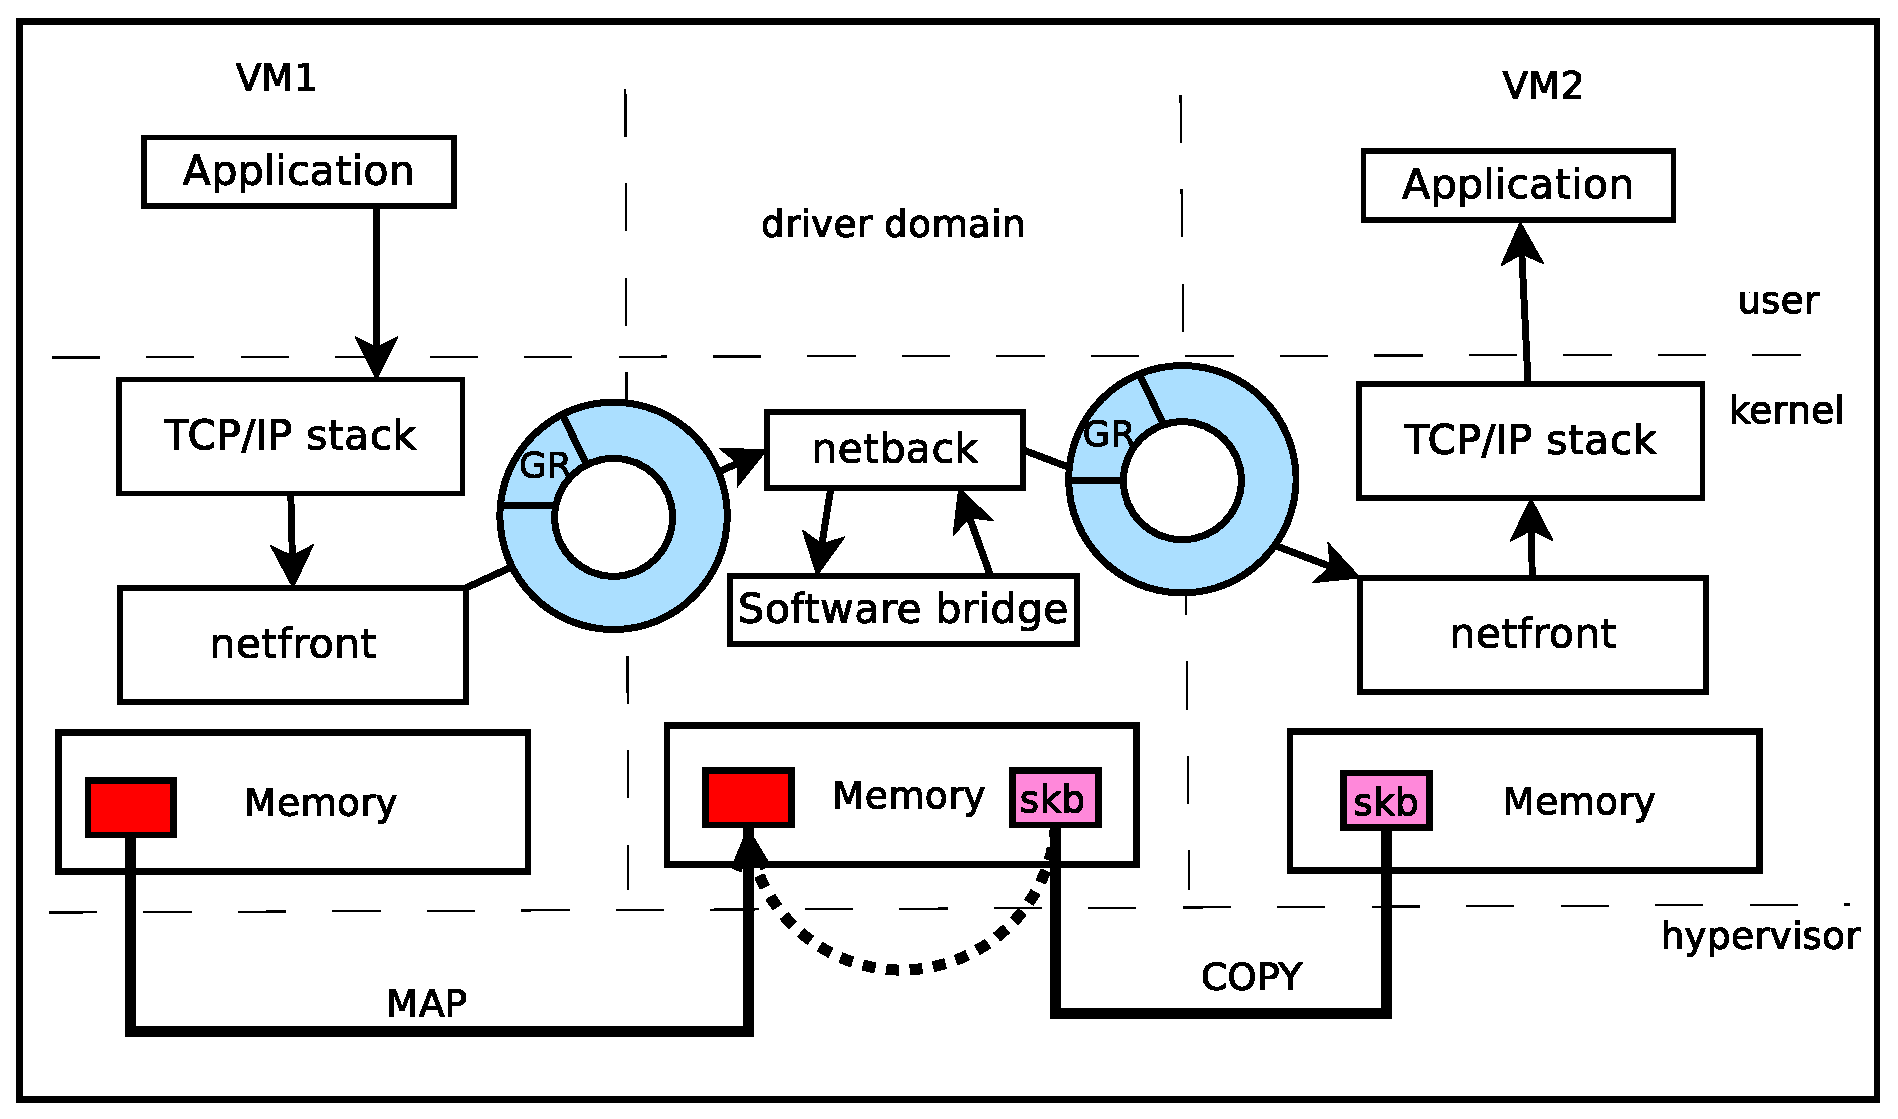
\includegraphics[width=\linewidth]{figures/netfront_netback.eps}
%Intra-node communication suffers from severe overheads mostly due to:
%\begin{itemize}
%\item inefficient data paths
%\item driver domain intervention in packet forwarding / handling
%\item driver domain intervention in packet forwarding / handling
%\item driver domain intervention in packet forwarding / handling
%\end{itemize}
\hspace{0.5em}\scalebox{.96}{
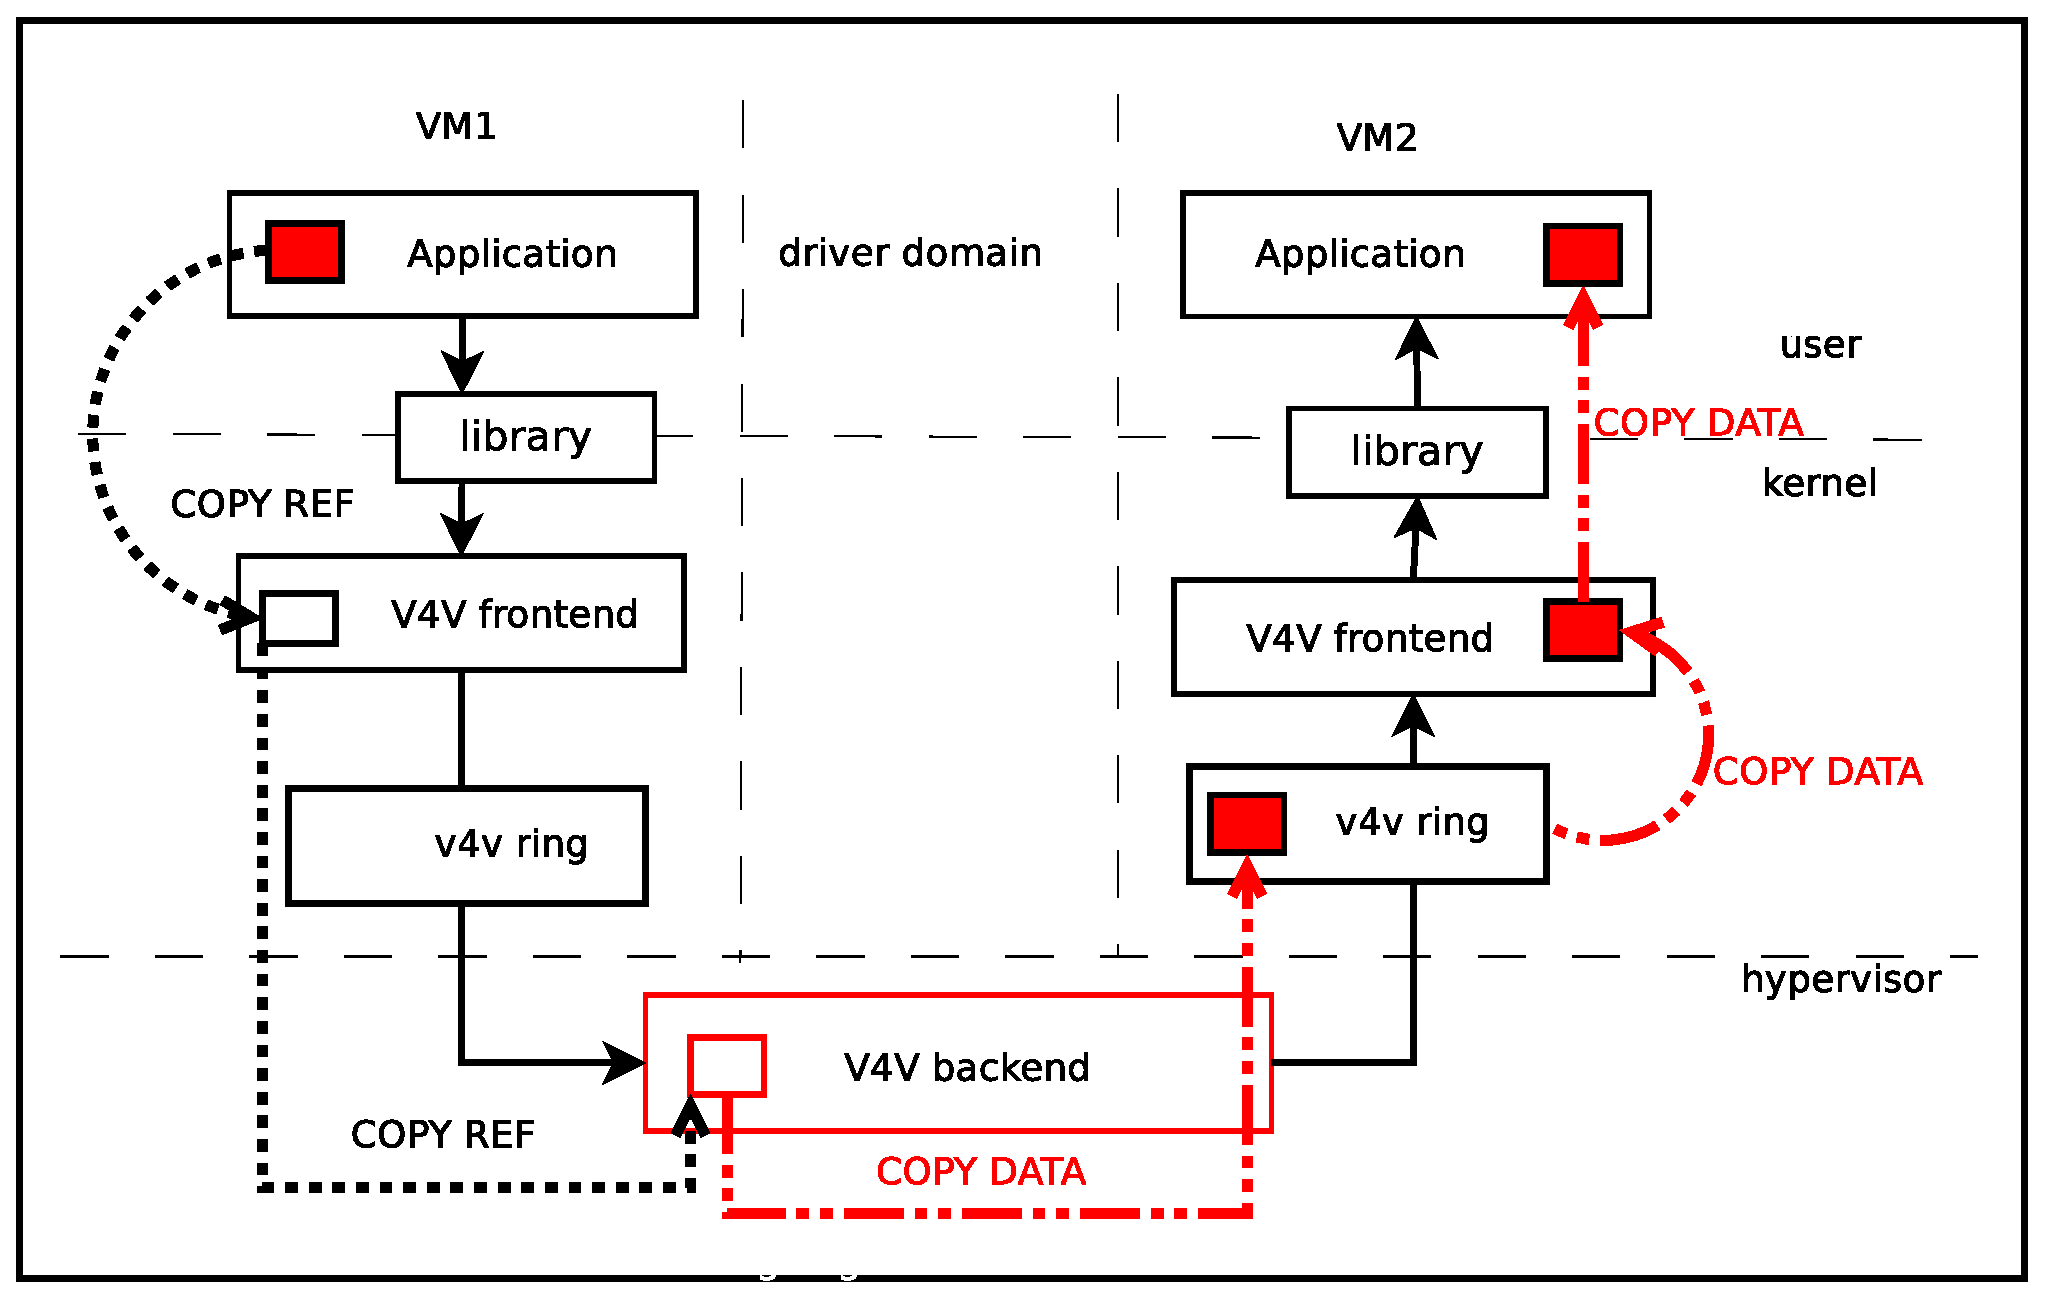
\includegraphics[width=\linewidth]{figures/v4vsockets.eps}
%\includegraphics[width=.5\linewidth]{}
  }
\end{multicols}
}

%%%%%%%%%%%%%%%%%%%%%%%%%%%%%%%%%%%%%%%%%%%%%%%%%%%%%%%%%%%%%%%%%%%%%%%%%%%%%%
  \headerbox{Contribution}{name=contribution,column=0, below=network path}{
%%%%%%%%%%%%%%%%%%%%%%%%%%%%%%%%%%%%%%%%%%%%%%%%%%%%%%%%%%%%%%%%%%%%%%%%%%%%%%
$\Rightarrow$ We introduce V4VSockets, an efficient, socket-compliant,
high--performance intra-node communication framework.

$\Rightarrow$ efficient data path. Data are copied from~/~to the VM kernel memory
without the need to share pages between VMs.

$\Rightarrow$ no intermediary VM (driver domain), so no scheduling implications are involved. 

$\Rightarrow$ We evaluate V4VSockets using generic micro-benchmarks and compare
it to conventional communication paths. We find that V4VSockets outperforms the
generic method of intra-node communication and scales efficiently with a large
number of VMs both in terms of throughput as well as latency.

$\Rightarrow$ We present a real-life use case: we deploy an HPC application
stencil over rCUDA, a remote GPU execution stack over V4VSockets.

\vspace{1em}
}


%%%%%%%%%%%%%%%%%%%%%%%%%%%%%%%%%%%%%%%%%%%%%%%%%%%%%%%%%%%%%%%%%%%%%%%%%%%%%%%%
%% \headerbox{Acknowledgements}{name=acknowledgements,column=0,above=bottom}{
%%%%%%%%%%%%%%%%%%%%%%%%%%%%%%%%%%%%%%%%%%%%%%%%%%%%%%%%%%%%%%%%%%%%%%%%%%%%%%%%
%%  \small
%%%  \hspace{1em}
%%   The authors would like to thank Nikos Nikoleris, Elisavet Kozyri and Stratos Psomadakis for their usefull contributions to this work.
%%\vspace{0.5em}
%%  }
%
%%%%%%%%%%%%%%%%%%%%%%%%%%%%%%%%%%%%%%%%%%%%%%%%%%%%%%%%%%%%%%%%%%%%%%%%%%%%%%%
 \headerbox{Preliminary results}{name=results,column=1,below=network path}{
%%%%%%%%%%%%%%%%%%%%%%%%%%%%%%%%%%%%%%%%%%%%%%%%%%%%%%%%%%%%%%%%%%%%%%%%%%%%%%%
%\setlength{\columnseprule}{1pt}
%\setlength{\columnsep}{13pt}
%\begin{multicols}{2}
\hspace{0.5em}\scalebox{.990}{
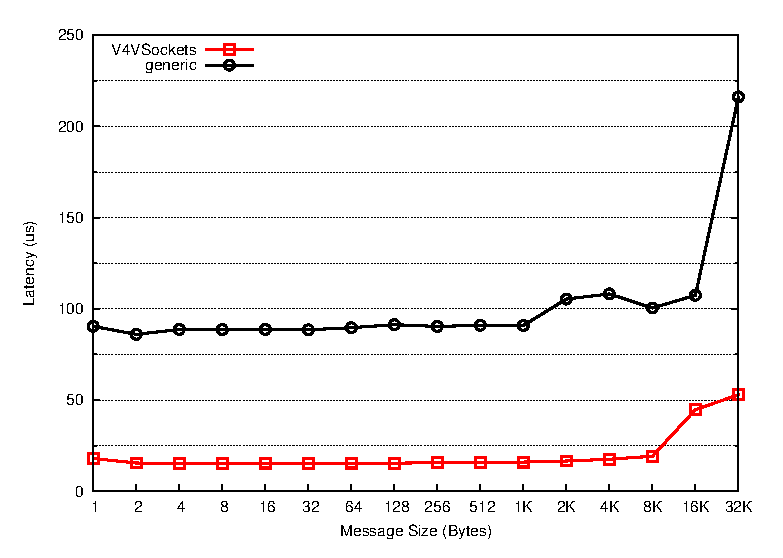
\includegraphics[width=\linewidth]{figures/v4v_lat.eps}}

V4VSockets improves the latency for small messages by 81\% compared to the
generic case. 
}


 \headerbox{Preliminary results (throughput)}{name=results2,column=2,below=network path}{
%\begin{multicols}{2}
\hspace{0.5em}\scalebox{.990}{
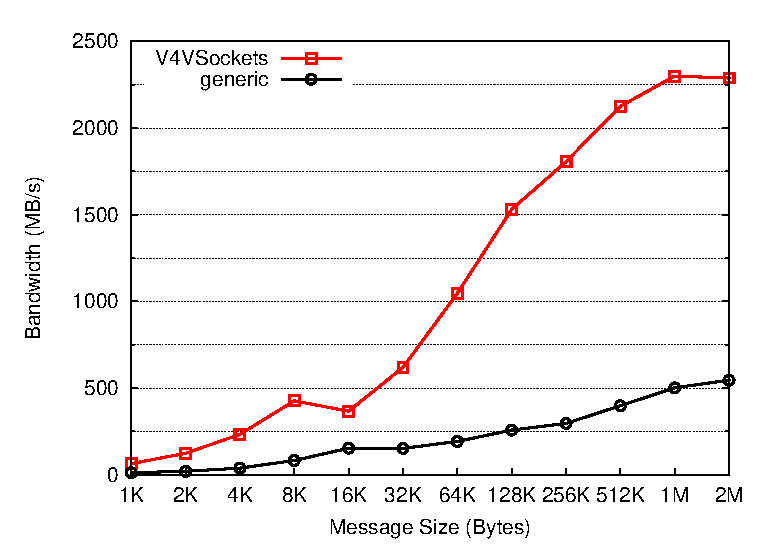
\includegraphics[width=\linewidth]{figures/v4v_bw.eps}}
%\begin{multicols}{2}
V4VSockets outperforms the default case for communication. V4VSockets is able
to achieve 2299 MB/s, 4.5x better than the split driver, which performs poorly
at 501 MB/s for 1 MB messages.
%\end{multicols}
%\begin{itemize}
%\item no page sharing
%\item no ethernet fragmentation
%\item No driver domain, no scheduling implications.
%\end{itemize}
%
%\end{multicols}

}

 \headerbox{GPU use case}{name=gpu,column=0,span=2,above=bottom}{
\begin{multicols}{2} 

%\hspace{0.5em}\scalebox{.990}{
%}
This experiment includes the following procedure: two copies of the input
matrices from node's main memory to GPU device memory, the product execution on
the GPU and finally one copy of the output matrix back to main memory. % The
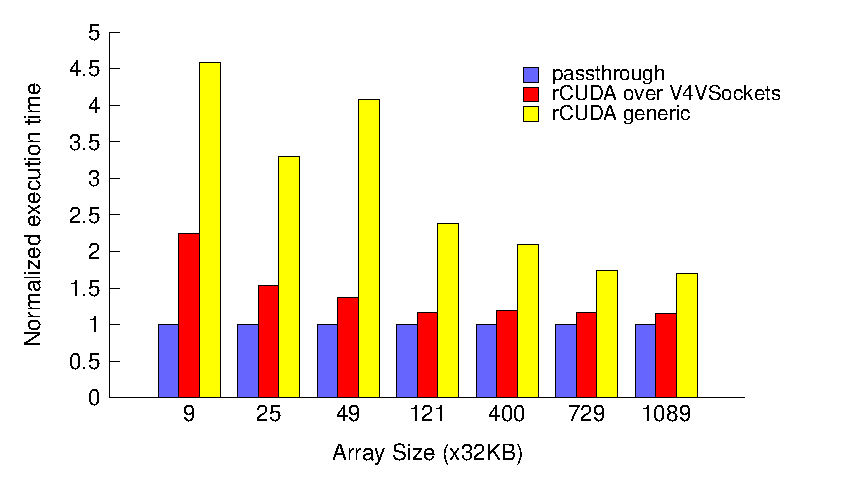
\includegraphics[width=\linewidth]{figures/total_cublas_time.eps}
%normalized total time of execution of the matrix-matrix product benchmark is
%depicted in the Figure on the left.
%\begin{multicols}{2}
%\hspace{0.5em}\scalebox{.990}{
%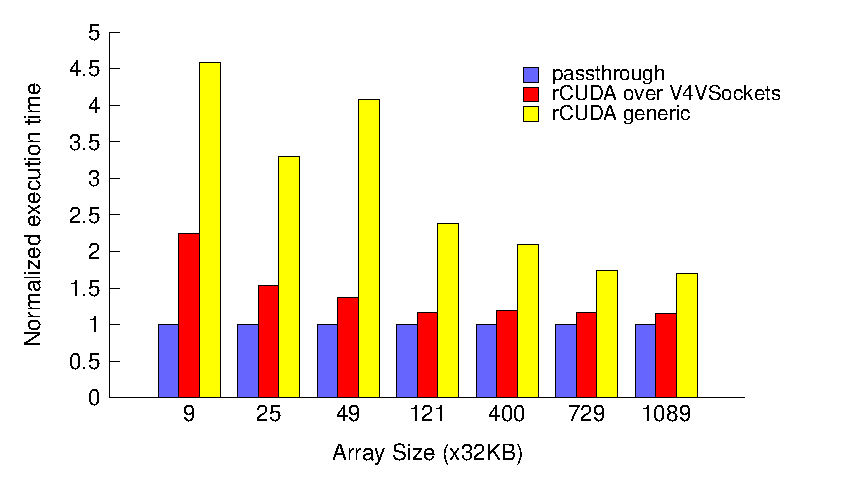
\includegraphics[width=\linewidth]{figures/total_cublas_time.eps}}

\hspace{0.5em}\scalebox{.990}{
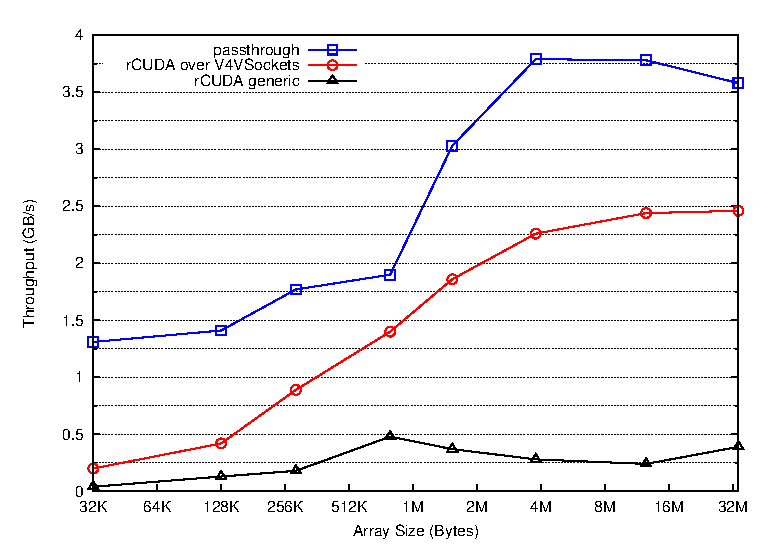
\includegraphics[width=\linewidth]{figures/matrixA_cublas_throughput.eps}
}

To elaborate more on the impact of V4VSockets to the improvement in the
execution time, we plot the throughput achieved when copying one of the input
matrices from the machine's main memory to the GPU device memory (essentially
this is a \texttt{cudamemcpy()} call).
\end{multicols}

%We observe that the peak throughput is 3.79 GB/s in our baseline experiment,
%while the respective throughput in the remote V4VSockets case is 2.46 GB/s.
%However, for a matrix size of 34 MB (2112 x 4224 float type elements)
%V4VSockets outperforms the generic case by a factor of 7 (0.35 GB/s).
%\end{multicols}

\vspace{1em}
}

%%%%%%%%%%%%%%%%%%%%%%%%%%%%%%%%%%%%%%%%%%%%%%%%%%%%%%%%%%%%%%%%%%%%%%%%%%%%%%%
%  \headerbox{Open Challenges}{name=questions,column=0,span=1,below=contribution}{
%%%%%%%%%%%%%%%%%%%%%%%%%%%%%%%%%%%%%%%%%%%%%%%%%%%%%%%%%%%%%%%%%%%%%%%%%%%%%%%
%    
%\textit{Higher-level parallel frameworks}: Our protocol implements simple RDMA semantics
%(READ, WRITE). We are in the process of extending its capabilities to support
%higher-level frameworks for application parallelism such as MPI or MapReduce.
%
%\textit{Performance}: Efficient I/O device sharing and support in Virtualized
%environments does not appear to be sufficiently mature. Even in full
%virtualization setups, many I/O devices have to be exported as emulated devices
%to VMs. %In this work, we observe suboptimal performance when transferring data
%%from VMs to network using common generic approaches (such as TCP/IP over 10GbE
%%adapters), while at the same time CPU cores were busy multiplexing accesses to
%%the hardware. 
%%In order to be able to deploy HPC applications in VM
%%environments, we have to take into account overheads imposed by Virtualization
%%layers and eliminate them. 
%
%\textit{Hardware Offloading}: Our prototype implementation consists of a frontend and a
%backend in the Xen virtualization platform. We show that while in the frontend
%part (VM) CPU time is negligible and agnostic to varying message sizes, there
%is still some CPU time spent in the Driver domain that can potentially reduce
%the performance of the entire system. This issue could be resolved by
%offloading this thin protocol layer to a hardware device, capable of performing
%DMA transfers and simple protocol processing. 
%%In addition to that, using SR-IOV
%%techniques with this custom device can lead to a VM-capable, high-performance
%%interconnection architecture over 10G Ethernet, comparable to VIA
%%Myrinet/Infiniband for virtualized environments. %To this end, we are in the
%%process of evaluating our approach in a custom, programmable controller
%%equipped with a 10GbE interface. We aspire to alleviate all CPU overheads
%%associated with protocol processing and propose optimizations that can achieve
%%near-native performance.
%
%\textit{Decoupling HPC from the Privileged Guest}: While a hardware approach, as
%mentioned above, could resolve CPU time issues, 
%we would like to examine the
%possibility of decoupling all HPC network-related issues to a different domain.
%This way, overheads associated with world switches and interrupt handling can
%be alleviated. We plan on evaluating this idea based on Xen stub domains, using
%modular networking components that can be easily implemented and optimized.
%   
%  }

\end{poster}

\end{document}
